\chapter{Esperimenti}
\section*{Setup testing}
Come anticipato precedentemente, il modello scelto ha un'architettura simile a quella di LeNet-5. Trattandosi di un task di classificazione vicino a quello del riconoscimento di cifre scritte a mano, la scelta di un'architettura ispirata a LeNet-5 è stata naturale, essendo consolidata per questo tipo di problemi.
Sono state comunque effettuate delle modifiche rispetto alla classica architettura sopra citata, sia per adattarla alle features del nostro task di classificazione (che prevedono un paio di input in più), sia per poter ottenere risultati migliori in fase di training (aggiungendo un paio di layer di dropout).
\\
Per poter ottenere la miglior combinazioni di iperparametri, sono stati effettuati diversi esperimenti, variando \emph{learning rate}, \emph{batch size}, \emph{dropout rate}, \emph{momentum} e \emph{numero di epoche}.
Per ognuna delle varianti negli iperparametri nella fase di training, viene generato un log TensorBoard che contiene le coppe di \emph{Loss} e \emph{Accuracy} in entrambi i dataset di training e validation. Inoltre, vengono salvati i pesi al termine delle epoche, utile per poterli ricaricare successivamente.
Di seguito vengono evidenziati gli esperimenti effettuati.

\section{Exps 1}
Il primo esperimento prevede l'iterazione di una griglia di parametri presenti all'interno di un file di configurazione. In particolare, la griglia prevede tutte le triple dei seguenti parametri nei corrispettivi range:
\begin{itemize}
    \item \textbf{Learning rate}: \{0.01, 0.001, 0.005, 0.0001, 0.0005\}
    \item \textbf{Dropout rate}: \{0.2, 0.3, 0.4, 0.5\}
    \item \textbf{Momentum}: \{0, 0.5, 0.9\}
\end{itemize}

Essendo un modello piuttosto piccolo, è stato ritenuto opportuno impostare una batch size di \textbf{2560}, garantendo un calcolo del gradiente più preciso comparato a una batch size piccola. Per semplicità, il numero di epoche è fissato a 50.

Questo approccio di \emph{grid search}, per quanto semplice, potrebbe già restituire dei risultati approssimativi sui range più opportuni per risolvere il problema, rendendo possibile ulteriori esperimenti nei range vicini alla tripla migliore. 

\begin{figure}[htbp]
    \centering
    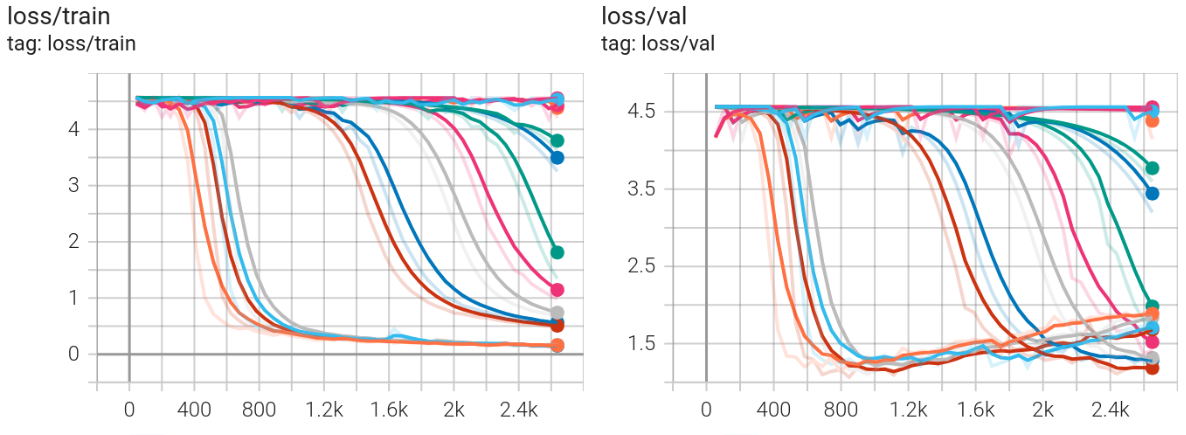
\includegraphics[width=0.8\textwidth]{images/exps1_loss.png}
    \caption{Loss Exps 1}
    \label{fig:exps1_loss}
\end{figure}

Durante la fase di training si è notato come i tempi di training siano dilatati, rendendo questo approccio inefficiente. Inoltre, a colpo d'occhio, durante l'iterazione dei vari iperparametri, si è notato come le prestazioni del modello fossero parecchio scadenti. Qualche training terminava in overfitting evidente, mentre altri sembravano non convergere entro le 50 epoche.

Per queste ragioni, senza ultimare il training con tutte le permutazioni, si è preferito procedere per via iterativa, come approfondito nella sezione successiva.

\section{Exps 2}

La soluzione più efficiente per ottimizzare il flusso precedentemente configurato si è rilevato essere un processo iterativo con l'intervento umano che regola gli iperparametri più opportuni man mano che gli esperimenti avvengono.

\begin{figure}[htbp]
    \centering
    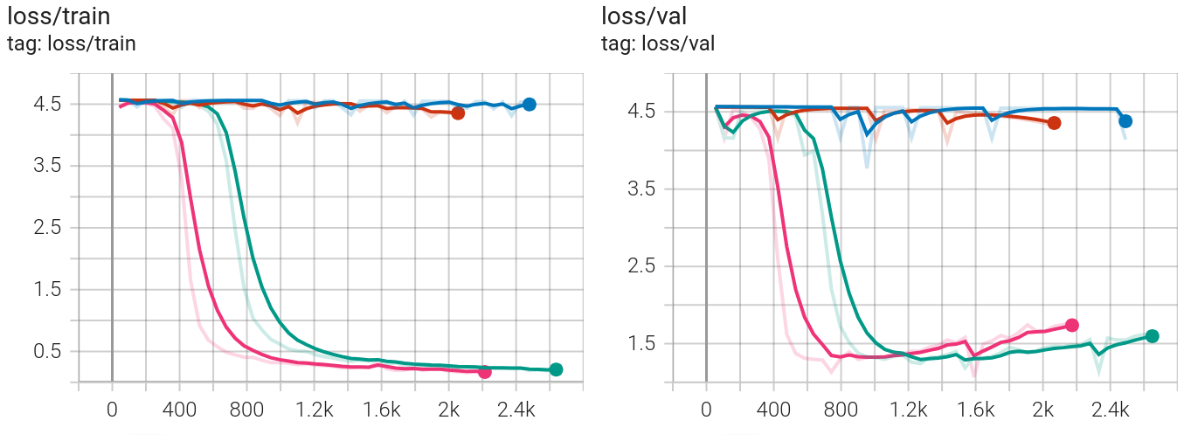
\includegraphics[width=0.8\textwidth]{images/exps2_loss.png}
    \caption{Loss Exps 2}
    \label{fig:exps1_loss}
\end{figure}

Il secondo esperimento evidenzia come, nonostante venga variato il dropout, il fenomeno di overfitting rimanga persistente.

Questo è probabilmente dovuto alla batch size parecchio grande, non consentendo di avere un grado di regolarizzazione sufficiente alto.


\section{Exps 3}

Per ovviare il problema della precedente sperimentazione, si è deciso di ridurre la batch size a \textbf{256}, consentendo di aumentare la regolarizzazione del modello.

Inoltre, un ulteriore tentativo di migliorare il modello si è configurato nella scelta di andare a riutilizzare i migliori pesi man mano che i parametri vengono cambiati. Questo consente di utilizzare un learning rate più basso quando in prossimità del minimo locale.

\begin{figure}[htbp]
    \centering
    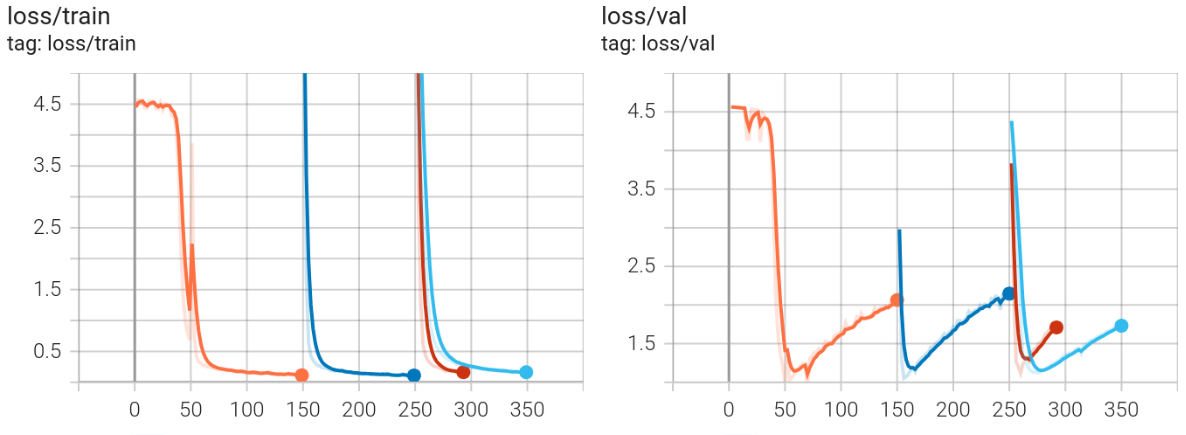
\includegraphics[width=0.8\textwidth]{images/exps3_loss.png}
    \caption{Loss Exps 3}
    \label{fig:exps1_loss}
\end{figure}

I tentativi mostrano uno scarso risultato nel combattere la varianza esibita dalle curve di train e loss.


\section{Exps 4 e 5}



\section{Valutazioni}
La valutazione sui singoli caratteri si articolano in diverse analisi:
\begin{itemize}
    \item Analisi score
    \item Curve Precision-Recall
    \item Matrice di confusione
\end{itemize}

\subsubsection*{Analisi degli Score}

Durante la fase di training, abbiamo monitorato l'\textit{accuracy} e la \textit{loss}. Al termine dell'addestramento, una volta fissati i pesi ottimali, abbiamo valutato le prestazioni del modello sul set di test. Per le migliori run di ciascun esperimento, sono state calcolate anche le metriche di \textbf{precision}, \textbf{recall} e \textbf{F1-score}, oltre all'\textbf{accuracy}, al fine di ottenere una valutazione più completa del comportamento del modello.

I risultati ottenuti per ciascuno dei cinque esperimenti condotti sono riassunti nella tabella seguente:

\subsubsection*{Risultati}
\begin{table}[H]
\centering
\begin{tabular}{c|c|c|c|c}
\textbf{Esperimento} & \textbf{Accuracy} & \textbf{Precision} & \textbf{Recall} & \textbf{F1-score} \\
\hline
1 & 0.85 & 0.82 & 0.80 & 0.81 \\
2 & 0.86 & 0.83 & 0.82 & 0.82 \\
3 & 0.88 & 0.85 & 0.84 & 0.84 \\
4 & 0.89 & 0.86 & 0.85 & 0.85 \\
5 & \textbf{0.91} & \textbf{0.89} & \textbf{0.88} & \textbf{0.88} \\
\end{tabular}
\caption{Metriche di valutazione sui cinque esperimenti.}
\label{tab:score_analysis}
\end{table}

Dall'analisi della tabella si può osservare come l'esperimento 5 abbia ottenuto le migliori prestazioni su tutte le metriche considerate.

\subsubsection*{Curve Precision-Recall}
Le curve Precision-Recall (PR) consentono di analizzare il bilanciamento tra \emph{precision} e \emph{recall} nelle predizioni del modello, mostrando quanto esso riesca a mantenere alta la precisione man mano che aumenta la quantità di caratteri correttamente riconosciuti. Un indicatore sintetico della qualità complessiva è l'area sotto la curva (AUC-PR), che risulta tanto più elevata quanto migliore è la capacità del modello di conciliare accuratezza e sensibilità nel riconoscimento dei caratteri.

\subsubsection*{Risultati}
In Figura~\ref{fig:pr_curves} sono riportate le curve per un sottoinsieme rappresentativo di classi non confondibili.

\begin{figure}[htbp]
    \centering
    \begin{subfigure}[t]{0.32\textwidth}
        \centering
        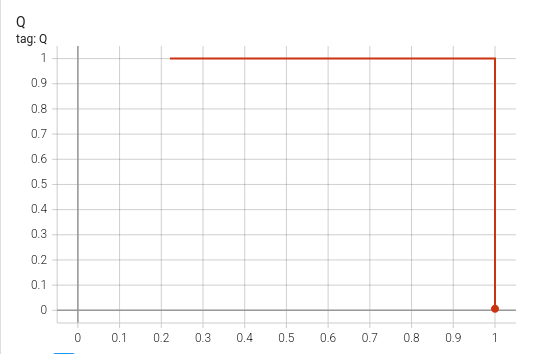
\includegraphics[width=\textwidth]{images/pr_curve1.png}
        \caption{PR-curve \{s\}}
    \end{subfigure}
    \begin{subfigure}[t]{0.32\textwidth}
        \centering
        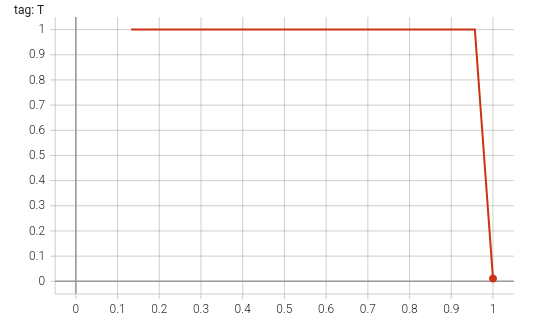
\includegraphics[width=\textwidth]{images/pr_curve2.png}
        \caption{PR-curve \{v\}}
    \end{subfigure}
    \begin{subfigure}[t]{0.32\textwidth}
        \centering
        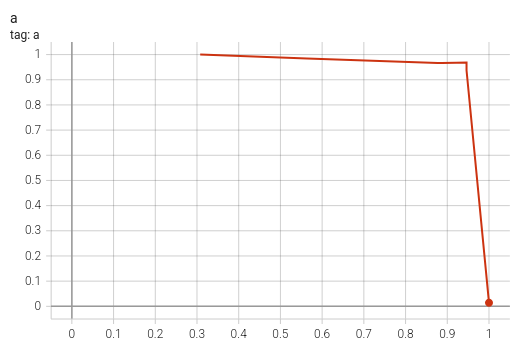
\includegraphics[width=\textwidth]{images/pr_curve3.png}
        \caption{PR-curve \{w\}}
    \end{subfigure}
    \caption{PR-curves per caratteri non confondibili}
    \label{fig:pr_curves}
\end{figure}

Nel complesso, il modello mostra buone prestazioni, con curve PR ampie e stabili per la maggior parte delle classi.

Tuttavia, alcune classi risultano più problematiche. Come visibile in Figura~\ref{fig:pr-confondibili}.

\begin{figure}[htbp]
    \centering
    \begin{subfigure}[t]{0.32\textwidth}
        \centering
        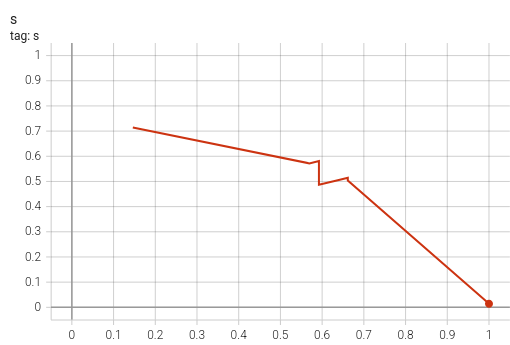
\includegraphics[width=\textwidth]{images/pr_curve_conf1.png}
        \caption{PR-curve \{s/S\}}
    \end{subfigure}
    \begin{subfigure}[t]{0.32\textwidth}
        \centering
        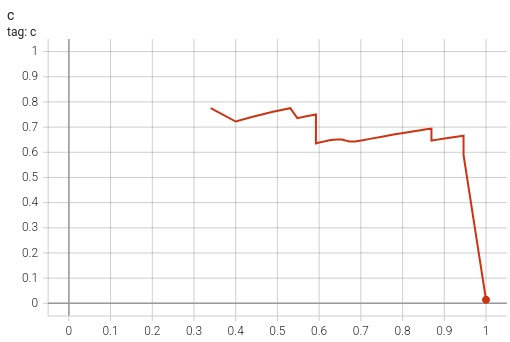
\includegraphics[width=\textwidth]{images/pr_curve_conf2.png}
        \caption{PR-curve \{w/W\}}
    \end{subfigure}
    \begin{subfigure}[t]{0.32\textwidth}
        \centering
        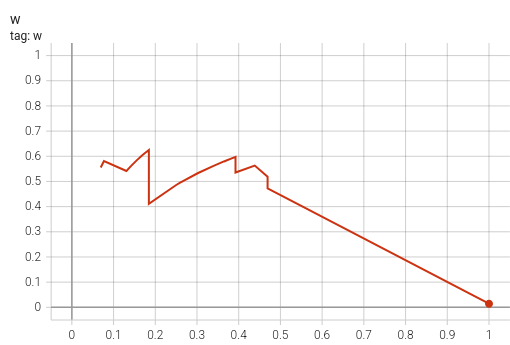
\includegraphics[width=\textwidth]{images/pr_curve_conf3.png}
        \caption{PR-curve \{w/W\}}
    \end{subfigure}
    \caption{PR-curves per caratteri confondibili}
    \label{fig:pr-confondibili}
\end{figure}

Per valutare l'impatto della distinzione tra maiuscole e minuscole, è stata ripetuta l'analisi ignorando il case. Come mostrato in Figura~\ref{fig:pr-ignore}, l'area sotto la curva migliora sensibilmente, suggerendo che una parte consistente degli errori è dovuta a una difficoltà del modello nel distinguere il case piuttosto che a un'incapacità di riconoscere la forma del carattere.
\begin{figure}[htbp]
    \centering
    \begin{subfigure}[t]{0.32\textwidth}
        \centering
        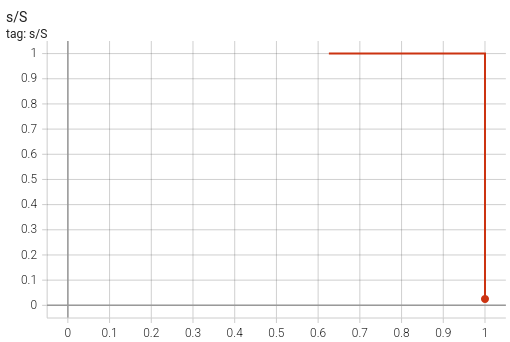
\includegraphics[width=\textwidth]{images/pr_ignore1.png}
        \caption{PR-curve \{s/S\}}
    \end{subfigure}
    \begin{subfigure}[t]{0.32\textwidth}
        \centering
        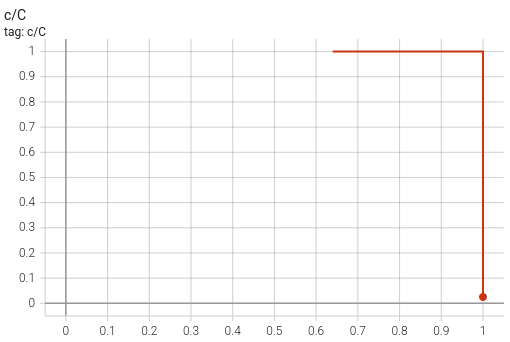
\includegraphics[width=\textwidth]{images/pr_ignore2.png}
        \caption{PR-curve \{c/C\}}
    \end{subfigure}
    \begin{subfigure}[t]{0.32\textwidth}
        \centering
        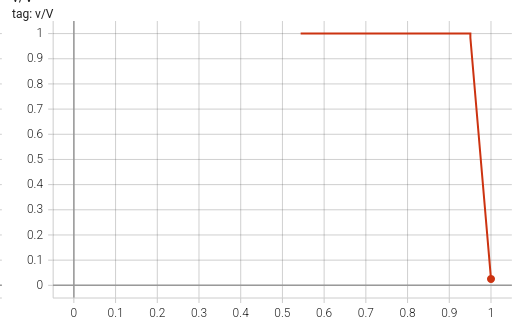
\includegraphics[width=\textwidth]{images/pr_ignore3.png}
        \caption{PR-curve \{v/V\}}
    \end{subfigure}
    \caption{PR-curves ignorando il case}
    \label{fig:pr-ignore}
\end{figure}

Infine, un esempio emblematico è riportato in Figura~\ref{fig:pr_strange}, dove, nonostante l'ignoramento del case, le prestazioni del modello rimangono insoddisfacenti.

\begin{figure}[htbp]
    \centering
    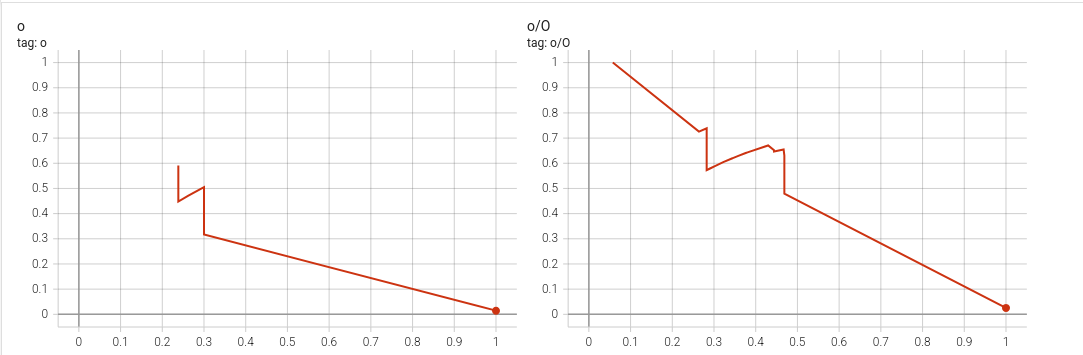
\includegraphics[width=0.65\textwidth]{images/pr_strange.png}
    \caption{PR-curve \{o\}}
    \label{fig:pr_strange}
\end{figure}

In assenza di un modello che tenga conto del contesto semantico, risulta difficile discriminare correttamente questi caratteri.

\subsection{Matrice di Confusione}

La matrice di confusione fornisce una rappresentazione dettagliata degli errori di classificazione commessi dal modello. Ogni cella \((i, j)\) della matrice indica il numero di volte in cui un carattere appartenente alla classe \(i\) è stato classificato come \(j\).

\begin{figure}[htbp]
    \centering
    \includegraphics[width=0.5\textwidth]{images/confusion_matrix.png}
    \caption{Matrice di confusione}
    \label{fig:confusion_matrix}
\end{figure}

Come si può osservare in Figura~\ref{fig:confusion_matrix}, la diagonale principale della matrice è ben marcata, a indicare che la maggior parte delle predizioni corrisponde correttamente alla classe attesa. Le deviazioni più significative dalla diagonale si concentrano principalmente tra le classi confondibili.

Analogamente a quanto fatto per le PR-curves, è stata condotta un'analisi ignorando il case. Come mostrato in Figura~\ref{fig:confusion_matrix_case_insensitive}, questa analisi evidenzia una riduzione significativa degli errori di classificazione, confermando che una parte consistente delle confusioni è attribuibile a questo tipo di confusioni.

\begin{figure}[htbp]
    \centering
    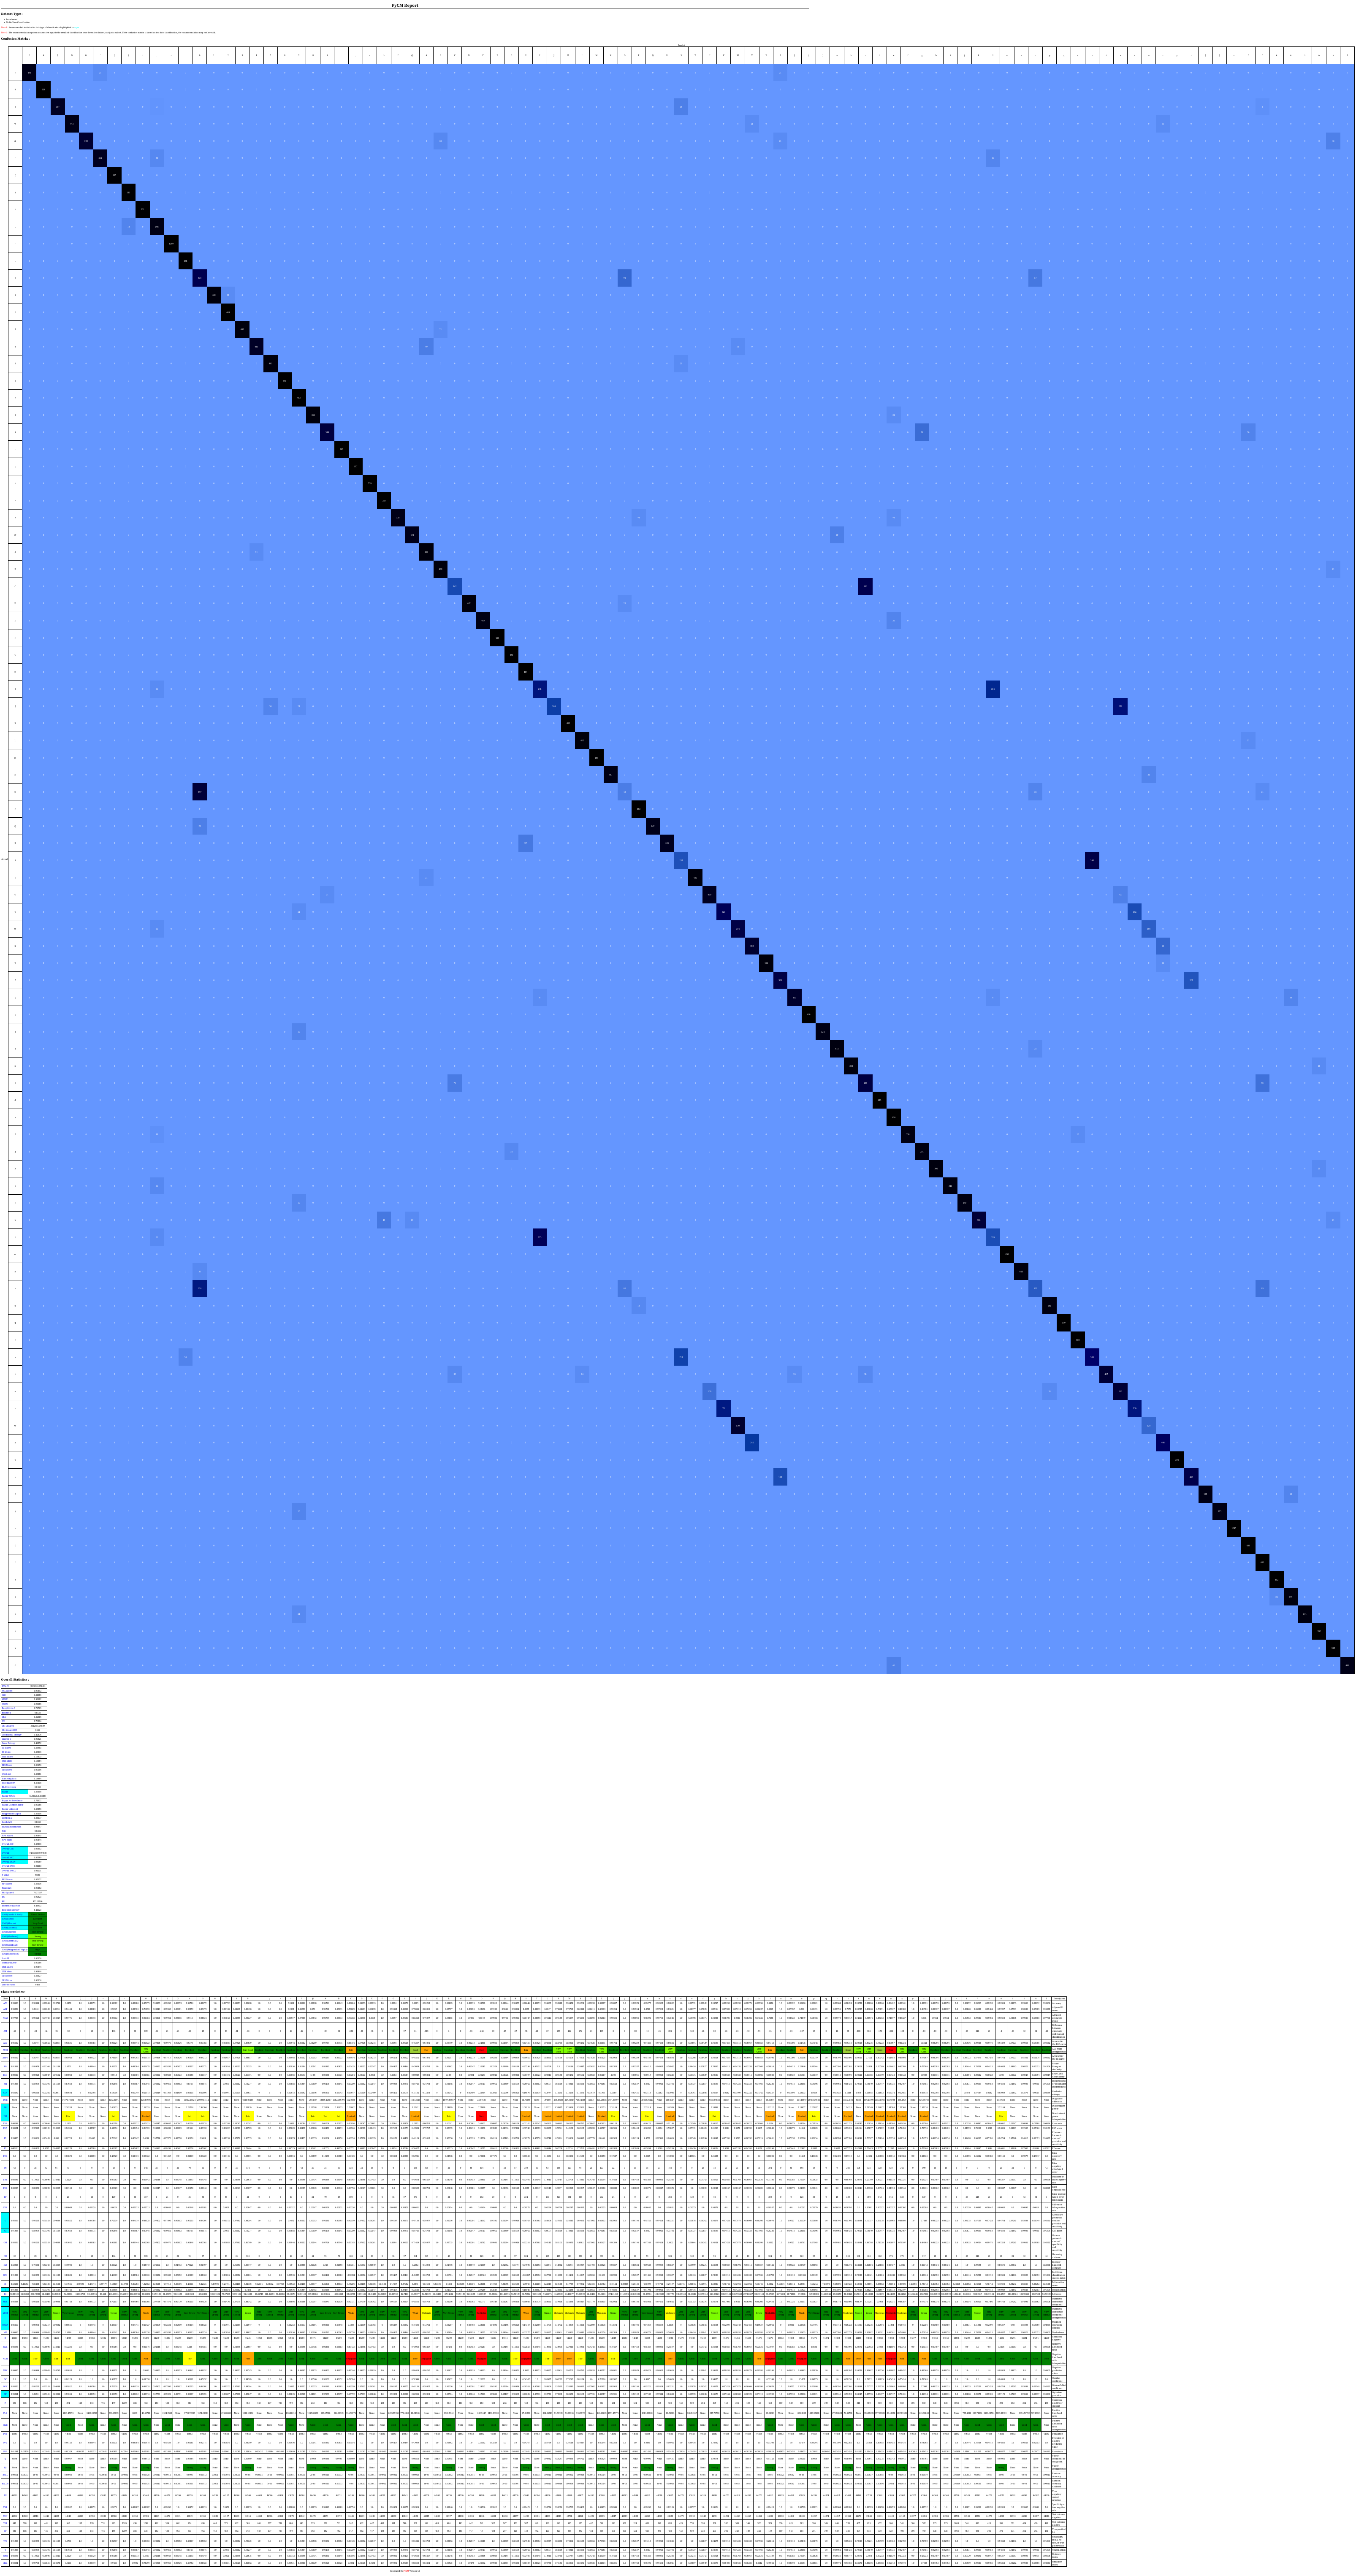
\includegraphics[width=0.5\textwidth]{images/confusion_matrix_case.png}
    \caption{Matrice di confusione ignorando il case}
    \label{fig:confusion_matrix_case_insensitive}
\end{figure}

Nel repository del progetto sono disponibili le matrici di confusione completa sotto forma di report HTML.

\subsection{Valutazione parole}
\label{sec:valutazione-stringhe}

Per l'analisi a livello di parola sono state adottate due metriche principali:
\begin{enumerate}
    \item Distanza di edit (\emph{Levenshtein distance \footnote{V. I. Levenshtein, “Binary codes capable of correcting deletions, insertions and reversals,” \textit{Soviet Physics Doklady}, vol. 10, pp. 707-710, 1966.} });
    \item String Accuracy.
\end{enumerate}

\subsection{Distanza di edit}
La distanza di edit tra la parola riconosciuta e la parola ground-truth è stata calcolata per ciascun esempio, normalizzando il valore sulla lunghezza della parola.

Di seguito si riporta una tabella con le statistiche principali della distanza di edit normalizzata, calcolate separatamente per i due dataset.

\begin{table}[htbp]
    \centering
    \begin{tabular}{lcccc}
        \toprule
        Dataset                 & Min   & Max   & Mean  & Std   \\
        \midrule
        Stringhe casuali       & 0  & 41 & 5.42  & 22.04 \\
        Stringhe inglesi & 0  & 2195 & 57.22  & 27521.79 \\
        \bottomrule
    \end{tabular}
    \caption{Statistiche della distanza di edit normalizzata per i due dataset}
    \label{tab:edit_distance_stats}
\end{table}

Da questi risultati emergono alcuni comportamenti anomali del modello, in particolare una marcata difficoltà nell'elaborazione di font molto sottili. Come evidenziato in Figura~\ref{fig:thin_fonts_bboxes}, il modello fatica a rilevare correttamente i tratti dei caratteri sottili, principalmente a causa dei bounding box. I riquadri generati in questi casi limite risultano spesso mal posizionati o incompleti, compromettendo i dato in ingresso e ostacolando la corretta interpretazione del carattere.

\begin{figure}[htbp]
    \centering
    \begin{subfigure}[t]{0.45\textwidth}
        \centering
        
\includegraphics[width=\textwidth]{images/thin_font1.png}
        \caption{Immagine originale}
    \end{subfigure}
    \hfill
    \begin{subfigure}[t]{0.45\textwidth}
        \centering
        
\includegraphics[width=\textwidth]{images/thin_font1_preproc.png}
        \caption{Bounding box errato}
    \end{subfigure}

    \caption{Esempi di immagini problematiche con font sottili e relativi errori nei bounding box.}
    \label{fig:thin_fonts_bboxes}
\end{figure}

\begin{table}[htbp]
    \centering
    \begin{tabular}{|c|c|}
        \hline
        \textbf{Ground Truth} & \textbf{Output} \\
        \hline
        \texttt{PEj\%6DuZi8} & \texttt{[:.\ E-j\ :C:::\ :::\ [:::\ é...Z.\ !d} \\
        \hline
        \texttt{unzmu\#QRRu} & \texttt{é...\ eN.Z\ .-NP-N.\ é...@\ :::\textbackslash..\ [:\ [:\ é...} \\
        \hline
    \end{tabular}
    \caption{Esempi di riconoscimenti errati generati dal modello.}
    \label{tab:recognition_examples}
\end{table}

\textcolor{red}{INSERIRE analisi togliendo questi font????}

\subsection{String Accuracy}
La string accuracy è definita come la percentuale di stringhe riconosciute esattamente nella loro interezza:
\[
    \mathrm{StringAccuracy} = \frac{\text{numero di stringhe perfettamente riconosciute}}{\text{numero totale di immagini}}.
\]

Per una valutazione più dettagliata, sono state considerate le seguenti varianti di string accuracy, che tengono conto di diverse esigenze di confronto:

\begin{itemize}
    \item \textbf{Accuracy case sensitive (CS)}: confronto rigoroso che distingue tra maiuscole e minuscole;
    \item \textbf{Accuracy case insensitive (CI)}: confronto che ignora le differenze tra maiuscole e minuscole, utile per valutare la capacità di distinguere caratteri simili o confondibili;
    \item \textbf{Accuracy case sensitive senza spazi (CSNS)}: confronto che ignora gli spazi ma distingue tra maiuscole e minuscole, utile per valutare la capacità di riconoscimento senza considerare errori di spaziatura.
    \item \textbf{Accuracy case insensitive senza spazi (CINS)}: confronto che ignora sia il case sia gli spazi, utile per gestire eventuali errori di segmentazione o spaziatura

\end{itemize}

La tabella seguente riporta i valori di string accuracy per ciascuna casistica, calcolati separatamente sui due dataset degli screenshot.

\begin{table}[htbp]
    \centering
    \begin{tabular}{lcccc}
        \toprule
        Dataset & CS & CI & CSNS & CINS \\
        \midrule
        Stringhe casuali & 2.87 & 3.60 & 35.00 & 47.80 \\
        Stringhe inglesi & 3.93 & 9.13 & 13.33 & 34.27 \\
        \bottomrule
    \end{tabular}
    \caption{String Accuracy per dataset e casistica di confronto}
    \label{tab:string_accuracy_stats}
\end{table}

Gran parte degli errori riscontrati deriva dalle euristiche utilizzate nel post-processing, in particolare quelle relative alla generazione degli spazi tra le parole.  
Inoltre, è presente il problema delle lettere confondibili, come lo zero con la lettera “O” o la “I” con la “L”.  
Abbiamo quindi alleggerito la metrica CINS, escludendo questo tipo di errori dal conteggio.  
Come mostrato nella Tabella~\ref{tab:error_rates}, questa modifica consente una significativa riduzione del tasso di errore, in particolare nel caso delle stringhe casuali.

\begin{table}[htbp]
    \centering
    \begin{tabular}{lc}
        \toprule
        Dataset & CINS* \\
        \midrule
        Stringhe casuali & 53.00 \\
        Stringhe inglesi & 39.47 \\
        \bottomrule
    \end{tabular}
    \caption{Percentuale di errori dovuti a lettere confondibili per dataset}
    \label{tab:error_rates}
\end{table}